\subsection{M.PC.MS - Metriche Soddisfatte}

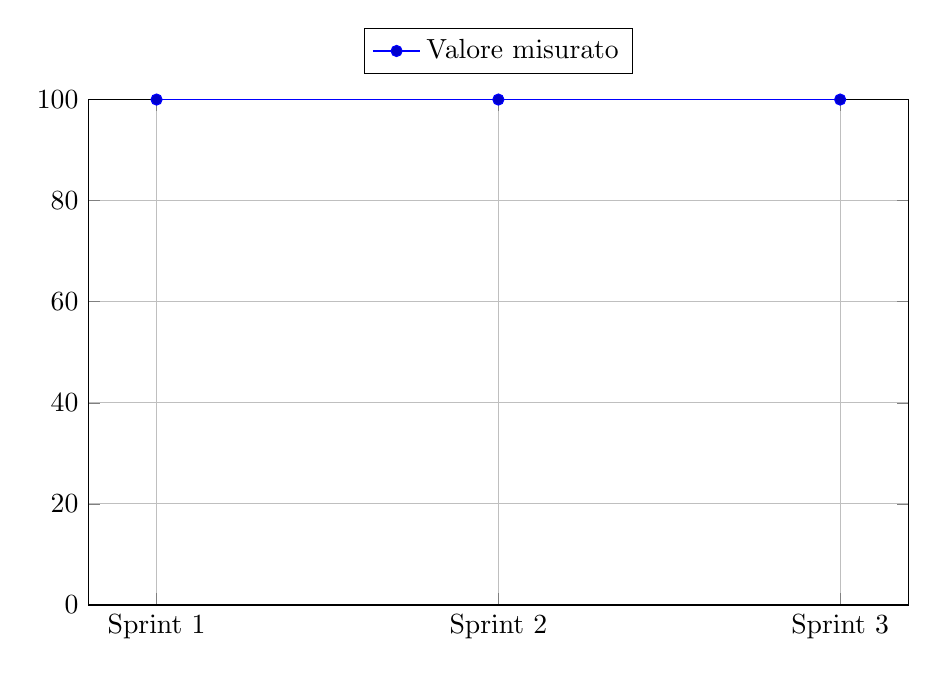
\begin{tikzpicture}
    \begin{axis}[
        width=12cm, height=8cm,
        ymin=0, ymax=100,
        xtick={1, 2, 3},
        xticklabels={Sprint 1, Sprint 2, Sprint 3},
        xlabel={},
        ylabel={},
        grid=major,
        legend style={at={(0.5,1.05)}, anchor=south, legend columns=-1},
    ]
    \addplot coordinates {(1, 100) (2, 100) (3, 100)};% ci vogliono prima i valori ammissibili e non, non sono sicuro della formula scritta su RTB/DocumentiInterni/NormeDiProgetto/Sezioni/ProcessiDiSupporto/Sottosezioni/AccertamentoQualità.tex riguardo le MetricheSoddisfatte
    \addlegendentry{Valore misurato}
    \end{axis}
\end{tikzpicture}

\subsection*{RTB}

\subsection*{PB}